\renewcommand{\theequation}{\theenumi}
\begin{enumerate}[label=\arabic*.,ref=\thesubsection.\theenumi]
\numberwithin{equation}{enumi}
\begin{figure}[!ht]
\centering
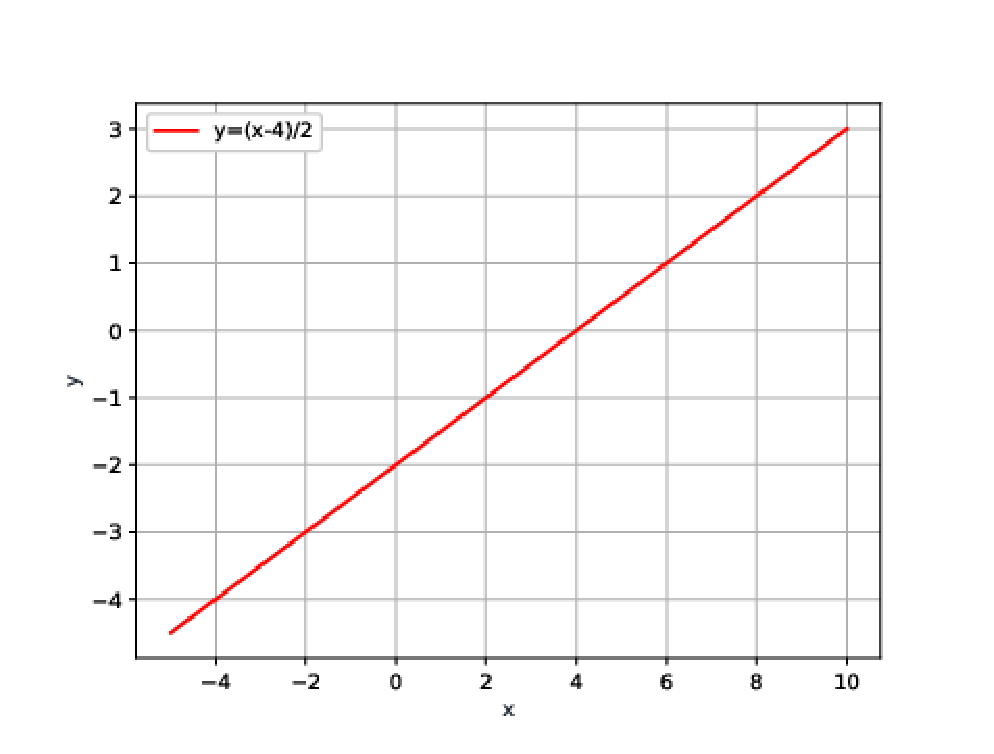
\includegraphics[width= \columnwidth]{./figs/line/lines_planes/fig.eps}
\caption{Line equation: y=(x-4)/2}
\end{figure}
\item If $\vec{x} = \myvec{x_1\\x_2}$, then the given equation can be expanded as,
\begin{align}
x_1 + 2x_2 = 4
\end{align}
\item Substitute given vectors from options in the above equation and check which will satisfy it.
\item Answer = $\myvec{4\\0}$
\item The python code for the figure 
\begin{lstlisting}
codes/line/lines_planes/lines_planes.py
\end{lstlisting}
\end{enumerate}